\chapter{React.js} \label{reactjs}
Dynaamisen komentokieli JavaScriptin suosion kasvun myötä syntyivät yhden sivun web-sovelluksien kehittämistä varten suunnitellut JavaScript-kehykset (engl. framework) ja -kirjastot (engl. library). Tällaisia maailmanlaajuisesti käytettyjä ja käytännöllisiksi tunnustettuja kehyksiä ja kirjastoja ovat esimerkiksi Angular JS, Vue.js ja React.js. Näistä kolmesta jälkimmäisin on tutkielman kirjoitushetkellä kasvanut maailmanlaajuisesti suosituimmaksi työkaluksi web-sovelluksien kehityksessä \cite{stackoverflowsurvey}.

React.js on Metan kehittämä ilmainen avoimen lähdekoodin JavaScript-kirjasto. Meta tunnettiin aiemmin nimellä Facebook. React kehitettiin yhden sivun web-sovelluksien kehittämistä varten. Kirjastoa ylläpitää aktiivisesti Metan lisäksi useasta henkilöstä ja yrityksestä koostuva yhteisö \cite{reactdocsteam}. Kirjastona React ottaa muita vastineitaan vähemmän kantaa erilaisten toiminnallisuuksien toteutustapoihin. Tästä syystä Reactin ympärille on muodostunut laaja kehittäjäyhteisö, joka kehittää ja julkaisee erilaisia kirjastoja, toteutustapoja ja ratkaisuja tyypillisiin ongelmiin \cite{rawatmahajan}. Tästä laajasta valikoimasta yksittäinen kehittäjä voi valita itselleen tai projektille soveltuvimman toteutustavan. Esimerkiksi reitittäminen toiminnallisuutena, joka on hyvin tyypillinen yhden sivun web-sovelluksessa, ei sisälly React-pakettiin, vaan löytyy muiden Reactin kehittäjätiimin ulkopuolisten kehittäjien julkaisemina ja ylläpitäminä kirjastoina. Vastaesimerkkinä laajemmin kantaa ottavasta JavaScript-kehyksestä on Angular JS, jossa esimerkiksi reitittäminen sisältyy kehykseen valmiina ominaisuutena. Vaikka React jättää monimutkaisemmat toiminnot kehittäjän harkintakyvyn varaan, on Reactissa kuitenkin selkeät raamit kehittämiselle. Esimerkiksi funktionaalisuudesta ja sovelluksen komponenttipohjaisuudesta ei voi Reactin käytössä välttyä.

%%
%% JSX
%%

\section{JSX}
\label{JSX}

JavaScript XML (JSX) on hyvin yleisesti React-sovelluksissa käytetty JavaScript-syntaksin jatke. JSX mahdollistaa React-elementtien luomisen deklaratiivisella ja yksinkertaistetulla syntaksilla. Visuaalisesti JSX muistuttaa pitkälti HTML-syntaksia.
\inputminted[bgcolor=black]{jsx.py:JsxLexer -x}{listaukset/jsx.js}
Myös lausekkeiden upottaminen on JSX:n avulla mahdollista. Sisällyttämällä minkä tahansa JavaScript-standardien mukainen lausekkeen aaltosulkeiden sisälle voidaan hyödyntää esimerkiksi muuttujaa tiedon esittämisessä. \cite{reactdocsjsx}
\inputminted[bgcolor=black]{jsx.py:JsxLexer -x}{listaukset/jsxexpression.js}

JSX:n käyttö ei ole kuitenkaan edellytys Reactin käytölle. React-sovelluksen kehittäminen onnistuu myös kirjoittamalla standardien mukaista Javascript-koodia. Tällöin React-elementin määritteleminen tulee tehdä Reactiin sisällytetyllä \texttt{createElement}-metodilla. \cite{reactdocswithoutjsx}
\inputminted[bgcolor=black]{jsx.py:JsxLexer -x}{listaukset/withoutjsx.js}
Vaikka JSX:n käyttö ei ole pakollista, on se hyvin suotavaa React-sovelluksen kehittämisessä.

%%
%% Komponentit
%%

\section{Komponentit}
\label{Komponentit}

Komponentit ovat oleellinen osa React-sovellusta. Ne toimivat rakennuspalikoina, joita yhdistelemällä sovellus muodostetaan \cite{reactdocscomponents}. Komponenttien avulla sovelluksen käyttöliittymä on mahdollista pilkkoa mielivaltaisen pieniin osiin, joita voidaan oikein toteutettuna käyttää toistuvasti sovelluksen eri osissa \cite{reactdocscomponents}. Komponentin pilkkominen osiin tuo erityisesti laajoihin kokonaisuuksiin selkeyttä ja läpinäkyvyyttä. Komponentin uusiokäytettävyyttä taas pidetään yleisesti hyvänä ominaisuutena. Uusiokäytettävien komponenttien suunnittelu ja kehitys vie aluksi aikaa, mutta säästää lopulta laajoissa sovellushankkeissa runsaasti aikaa ja resursseja \cite{holzmann}. Jos sovelluksessa on paljon toiminnaltaan samankaltaisia elementtejä tai saman ominaisuuden käyttötapauksia, voidaan kertaalleen laadittua komponenttia käyttää uudelleen useassa eri paikassa. Tällöin vältytään kyseisen komponentin kirjoittamiselta uudelleen joko osittain tai täysin.

Komponentin määrittelyyn on kaksi eri lähestymistapaa. Yksinkertaisin tapa määritellä komponentti on kirjoittaa (1) JavaScript-funktio. \cite{reactdocscomponents}
\inputminted[bgcolor=black]{jsx.py:JsxLexer -x}{listaukset/functioncomponent.js}
Komponentin voi toisaalta määritellä myös perusteellisemmin ES6-standardin mukaisella (2) JavaScript-luokalla. \cite{reactdocscomponents}
\inputminted[bgcolor=black]{jsx.py:JsxLexer -x}{listaukset/classcomponent.js}
Kun komponentti on määritelty, se voidaan ottaa käyttöön yksinkertaisella HTML-syntaksia muistuttavalla React-elementillä \texttt{<Komponentti />}. Elementit renderöidään loogisesti niiden esitysjärjestyksessä. 
\inputminted[bgcolor=black,highlightlines={4-5},highlightcolor=darkgray]{jsx.py:JsxLexer -x}{listaukset/componentusage.js}
Molemmat määrittelytavat ovat Reactin näkökulmasta yhtä päteviä. Funktiokomponenttien suosio on kuitenkin lisääntynyt kehittäjien keskuudessa niiden julkaisusta lähtien \cite{twilio}. Jopa itse Reactin takana olevan kehitystiimin tavoitteena on asteittain siirtyä luokkakomponenteista funktiokomponentteihin ajan kuluessa. \cite{reactdocshooks}

%%
%% Props
%%

\subsection{Props}
\label{Props}

Props eli properties on keino antaa komponentille tietoa käytettäväksi JavaScript-olion muodossa \cite{reactdocscomponents}. Propsit muistuttavat hyvin pitkälti funktiolle annettavia parametreja. Eräs tyypillinen propsien käyttötapaus on tilan jakaminen komponentilta toiselle. Tätä käsitellään tarkemmin tutkielman luvussa \ref{Tilan jakaminen muille komponenteille}. 

%%
%% Elinkaari
%%

\subsection{Elinkaari}
\label{Elinkaari}

Jokaisella React-komponentilla on oma elinkaarensa (engl. lifecycle). Elinkaari alkaa komponentin renderöinnistä ja päättyy lopulta komponentin irrotukseen dokumenttioliomallista (engl. document object model) \cite{reactdocsstate}. Komponentin elinkaaren avulla on mahdollista ajoittaa tiettyjen toimintojen suorittamista eri ajankohtiin ja tapahtumiin sovelluksen käynnistyksestä alkaen \cite{reactdocsstate}. Kuvasta \ref{fig:lifecycle} nähdään, miten komponentin elinkaari etenee komponentin kiinnittymisestä irtoamiseen. Tuntemalla ja tiedostamalla komponentin elinkaaren kehittäjä voi tehdä sovellukseen merkittäviä optimointeja, joilla on suora vaikutus sovelluksen suorituskykyyn ja käytettävyyteen. 
\begin{figure}[h]
\centering 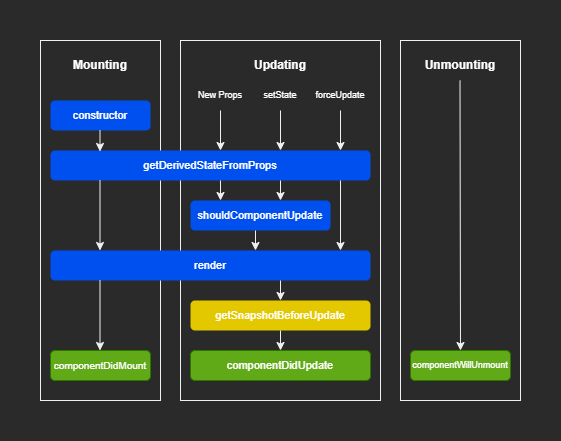
\includegraphics[width=1\textwidth]{kuvat/Elinkaari.png}
\caption{Graafinen esitys komponentin elinkaaresta.}
\label{fig:lifecycle} 
\end{figure}

%%
%% Tila
%%

\subsection{Tila}
\label{Tila}

Tila on läheisesti komponenttiin liittyvä käsite ja on tämän tutkielman näkökulmasta hyvin keskeisessä asemassa. Komponentilla voi olla yksi tai useampi tila, jota on mahdollista muuttaa esimerkiksi käyttäjän syötteen perusteella. Tilaa voidaan käyttää eri tarkoituksiin, kuten komponentin dynaamiseen esitystyyliin tai ehdolliseen näkyvyyteen. Mikäli komponentin palauttava \texttt{return}-lauseke on riippuvainen tilasta, joka voi muuttua, aiheutuu kuvan \ref{fig:component} mukaisesti kyseisen tilan muutoksesta komponentin päivittävä renderöinti \cite{reactandnative}. Käytännössä React vertaa edellistä DOM:in versiota nykyiseen ja suorittaa niiden osien päivittämisen, joihin muuttunut tilan arvo vaikuttaa. Tällöin vältytään koko sovelluksen päivittävältä renderöinniltä tilanteissa, joissa se ei ole ehdottoman tarpeellista. \cite{reactdocsrender}

\begin{figure}[h]
\centering 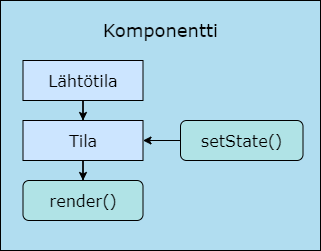
\includegraphics[width=0.5\textwidth]{kuvat/Komponentti.png}
\caption{Muutos tilassa aiheuttaa sitä käyttävän komponentin päivittävän renderöinnin.}
\label{fig:component} 
\end{figure}

%%
%% Hookit
%%

\section{Hookit}
\label{Hookit}

React julkaisi vuonna 2018 version 16.8 yhteydessä React Hooks -rajapinnan. Hookit ovat kokoelma erilaisia funktioita, jotka alkavat aina sanalla \texttt{use}. Hookit mahdollistavat React-komponentin ominaisuuksien käytön kirjoittamatta komponenttia luokkana \cite{reactdocshooks}. Esimerkkejä tällaisista ominaisuuksista ovat komponentin tilan määrittäminen ja päivittäminen sekä luvussa \ref{Elinkaari} mainitut elinkaarimetodit. Verrattuna luokkakomponentteihin funktiokomponentit yhdessä hookien kanssa ovat tyypillisesti helpommin luettavissa \cite[10]{buglreacthooks}. Ne myös vähentävät merkittävästi rutiininomaisen ja toistuvan koodin (engl. boilerplate code) kirjoittamista \cite{reactdocshooks} \cite[62]{reactandnative} \cite[11]{buglreacthooks}. Tutkielman myöhemmissä osissa tullaan käyttämään esimerkkeinä funktiokomponentteja yhdessä React Hooks -funktioiden kanssa luokkakomponenttien sijasta. 